\documentclass{report}
\usepackage[table,xcdraw]{xcolor}
\usepackage{tikz}
\usepackage{fancyhdr}
\usepackage[utf8]{vietnam}
\usepackage{hyperref} % Hyperlink
\usepackage{parskip}
\usepackage[left=2cm,right=2cm,top=2cm,bottom=2cm]{geometry}
\usepackage{minted}
\usetikzlibrary{calc}
\usepackage{titlesec} % Change section font
\usepackage{multirow}
\usepackage{graphicx}
\usepackage{algorithm,algorithmic}
\usepackage{multicol}
\usepackage{setspace}
\usepackage{pdfpages}
\usepackage{lscape}

% ========== [LANGUAGE] ==========
\def\lang{1} % 0 == English, 1 == Vietnamese

\ifnum\lang = 0
    \usepackage[english]{babel}
\fi
% ========== END OF [LANGUAGE] ==========





\begin{document}

% ========== [TITLE PAGE] ==========
\begin{titlepage}

\begin{tikzpicture}[overlay,remember picture]
\draw[line width=4pt]
    ($ (current page.north west) + (1cm,-1cm) $)
    rectangle
    ($ (current page.south east) + (-1cm,1cm) $);
\draw[line width=1.5pt]
    ($ (current page.north west) + (1.2cm,-1.2cm) $)
    rectangle
    ($ (current page.south east) + (-1.2cm,1.2cm) $);
\end{tikzpicture}


\begin{center}
% Upper part of the page
\ifnum\lang = 0
    \textbf{\Large UNIVERSITY OF SCIENCE}\\[0.2cm]
    \textbf{\Large FACULTY OF INFORMATION TECHNOLOGY}\\
\else
    \textbf{\Large TRƯỜNG ĐẠI HỌC KHOA HỌC TỰ NHIÊN}\\
    \textbf{\Large KHOA CÔNG NGHỆ THÔNG TIN}\\
\fi

% University Logo
\begin{figure}[!h]
    \centering
    
\includegraphics[width=8cm, height=8cm]{img/KHTN.png}
\end{figure}

% Title
\rule{\textwidth}{1pt} \\[0.4cm]
{\huge \bfseries ĐỒ ÁN CUỐI KÌ - NHÓM 10}\\[0.4cm]
\textsc{\Large VẬT LÝ CHO CNTT}
\rule{\textwidth}{1pt} \\[1cm]

% Student name
\begin{center}
    \textbf{\Large TRIỆU NHẬT MINH - 21127112}\\
    \textbf{\Large BÙI ĐỖ DUY QUÂN - 21127141}\\
    \textbf{\Large HOÀNG ĐỨC VIỆT - 21127203}\\[3cm]
\end{center}

% Advisor name
\begin{center}
    \ifnum\lang = 0
        \textbf{\Large Lecturers: \\[0.2cm]}
    \else
        \textbf{\Large Giảng viên hướng dẫn: \\[0.2cm]}
    \fi
    \Large{Cao Xuân Nam\\[0.2cm] Đặng Hoài Thương}
\end{center}
\vfill

% Bottom of the page
\ifnum\lang = 0
    \selectlanguage{english} 
\fi
{\large \today}
\end{center}
\end{titlepage}
% ========== END [TITLE PAGE] ==========





% ========== [HEADER AND FOOTER] ==========
\pagestyle{fancy}
\setlength{\headheight}{0.5cm}
\fancyhf{}
\lhead{\textbf{Đồ án cuối kì}}
\rhead{\textbf{Vật lý cho CNTT}}
\ifnum\lang = 0
    \rfoot{Page \thepage}
\else
    \rfoot{Trang \thepage}
\fi
% ========== END [HEADER AND FOOTER] ==========





% ========== [TABLE OF CONTENTS] ==========
\Large
\tableofcontents
\thispagestyle{fancy} % Fix footer and header
\vfill
\pagebreak
% ========== END [TABLE OF CONTENTS] ==========





% ========== [SECTION NUMBERING] ==========
\setcounter{secnumdepth}{5} % Section numbering depth 

\renewcommand\thesection{\arabic{section}} % Section start from 1,2,3...
\renewcommand\thesubsection{\thesection.\arabic{subsection}} % Subsection start from 1,2,3,...
\renewcommand\thesubsubsection{\alph{subsubsection}} 

\titleformat*{\section}{\Large\bfseries}
\titleformat*{\subsection}{\Large\bfseries}
\titleformat*{\subsubsection}{\Large\bfseries}
% ========== END [SECTION NUMBERING] ==========





% ========== [MAIN CONTENT] ==========
\section{Thông tin nhóm}
Thứ tự nhóm: Nhóm 10 \par
Danh sách thành viên:
\begin{itemize}
    \item Triệu Nhật Minh - 21127112
    \item Bùi Đỗ Duy Quân - 21127141
    \item Hoàng Đức Việt - 21127203
\end{itemize}

\section{Sản phẩm}
\subsection{Tên sản phẩm}
Thiết bị hỗ trợ sử dụng điện thông minh trong phòng

\subsection{Mô tả toàn chức năng của hệ thống}
\subsubsection{Hình ảnh sản phẩm}
Trong đồ án này, nhóm đã chọn thực hiện giả lập sản phẩm trên nền tảng \textbf{Wokwi} và dưới đây là hình ảnh các thiết bị và mạch nhóm đã thiết kế.
\begin{figure}[!h]
    \centering
    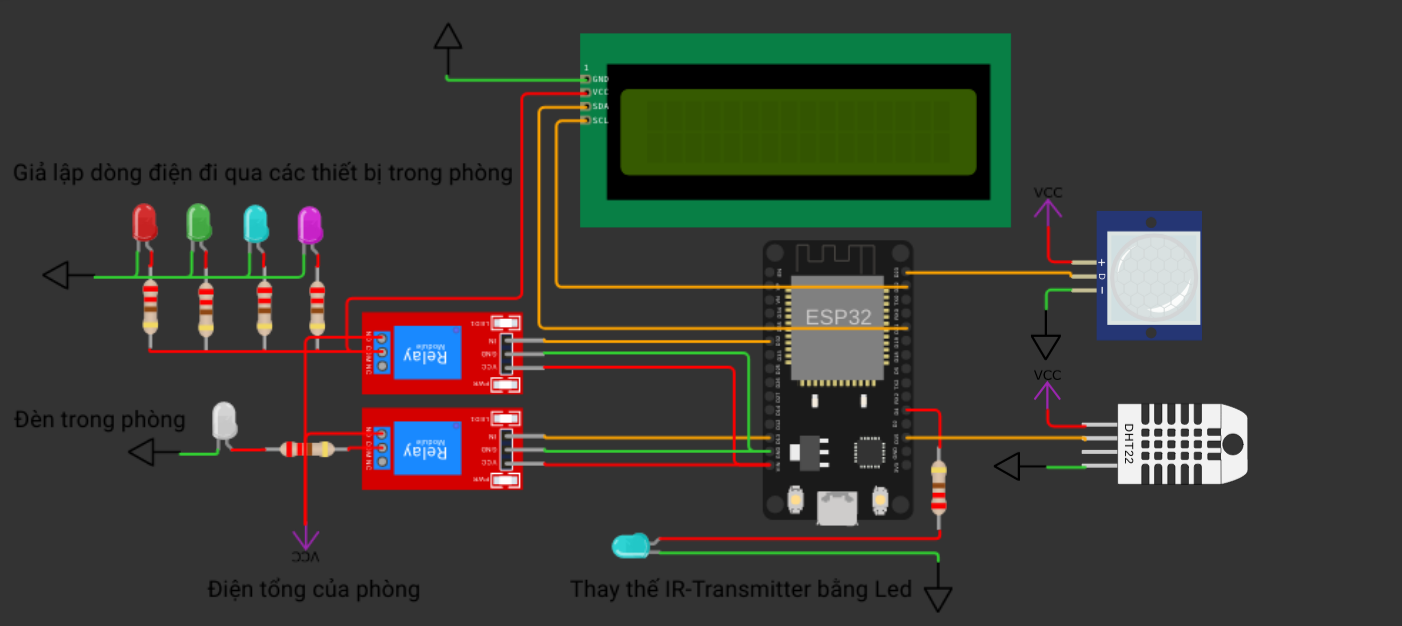
\includegraphics[width=\textwidth, keepaspectratio]{img/thiet_bi.png}
    \caption{Giả lập thiết bị hỗ trợ sử dụng điện thông minh trong phòng}
\end{figure}


\subsubsection{Các thiết bị sử dụng chính}
Dựa trên yêu cầu và qui định của đồ án cuối kì thì nhóm đã kết hợp các thiết bị cho sản phẩm ở hình trên như sau:
    \begin{itemize}
        \item Output: LCD, relay, IR-Transmitter
        \item Input: DHT22, cảm biến chuyển động (dạng hồng ngoại PIR).
        \item Board ESP32 có kết nối wifi.
    \end{itemize}

\subsubsection{Các thiết bị khác trong hình ảnh của sản phẩm}
\begin{itemize}
    \item Như đã được chú thích trong hình, vì không thể giả lập thiết bị IR-Transmitter nên nhóm đã sử dụng 1 bóng đèn led màu xanh dương (được nối trực tiếp với board ESP32). Khi bóng đèn led này chớp tắt tức là thiệt bị đã gửi tín hiệu hồng ngoại tới các thiết bị trong phòng.

    \item Bóng đèn led màu trắng chính là đèn chính trong phòng.

    \item 4 bóng đèn led còn lại được dùng để tương trưng cho các thiệt bị trong phòng đang có dòng điện đi qua. Nếu có điện trong phòng, 4 bóng đèn led này sẽ phát sáng tượng trưng cho việc các thiết bị điện trong phòng đang có điện.
\end{itemize}

\subsubsection{Tổng quát cách thức hoạt động của sản phẩm}
\begin{itemize}
    \item Sản phẩm này của nhóm sẽ nhận biết rằng người trong phòng hay không để thực hiện mở các thiết bị điện cần thiết. Thêm vào đó người dùng có thể kiểm soát được 2 chế độ "hoạt động" và "bảo vệ", trong đó: chế độ \textbf{"hoạt động"} sẽ giúp người dùng bật tắt thiết bị điện khi người dùng ra hay vào phòng, và chế độ \textbf{"bảo vệ"} sẽ ngắt cung cấp điện cho các thiết bị đồng thời cảnh báo người dùng khi có người vào phòng.

    \item Ngay khi khởi tạo, chế độ sẽ được mặc định là \textbf{"hoạt động"}, và các thiết bị trong phòng được cung cấp nguồn điện.

    \begin{figure}[!h]
        \centering
        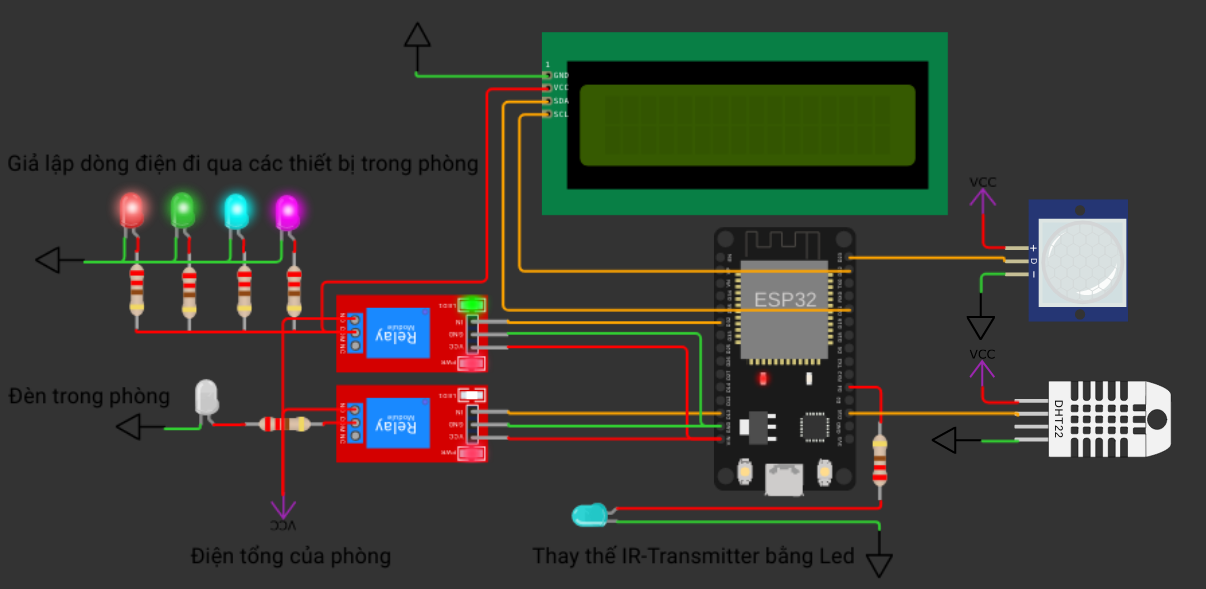
\includegraphics[width=\textwidth, keepaspectratio]{img/Khoi_tao.png}
        \caption{4 đèn led sáng tức là các thiết bị điện trong phòng đang được cung cấp điện}
    \end{figure}

    \pagebreak
    \item Khi có người bước vào phòng, \textbf{cảm biến chuyển động} sẽ nhận tín hiệu hồng ngoại và đèn trong phòng sẽ sáng, đồng thời trên màn hình \textbf{LCD} sẽ hiện lên thông tin về nhiệt độ, độ ẩm trong phòng.

    \begin{figure}[!h]
        \centering
        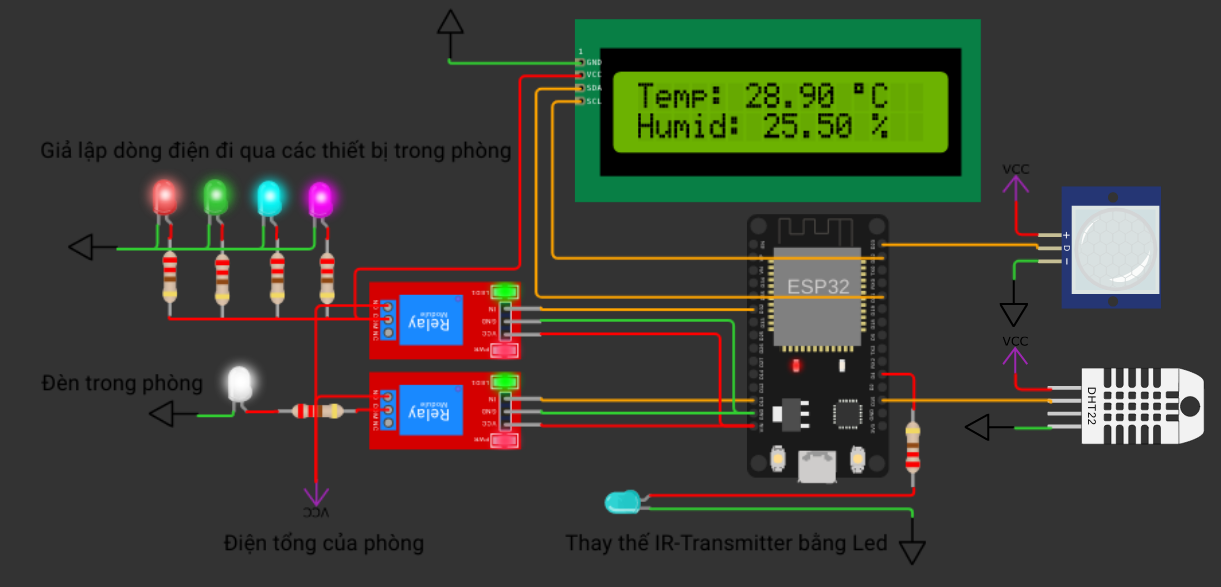
\includegraphics[width=\textwidth, keepaspectratio]{img/vao_phong.png}
        \caption{Đèn trong phòng sáng và thông tin được hiện trên màn hình LCD}
    \end{figure}

    \pagebreak
    \item Ngoài ra khi người dùng trong phòng và nhiệt độ lớn hơn 30°C thì máy lạnh sẽ được tự động mở thông qua thiết bị \textbf{IR-Transmitter}.

    \begin{figure}[!h]
        \centering
        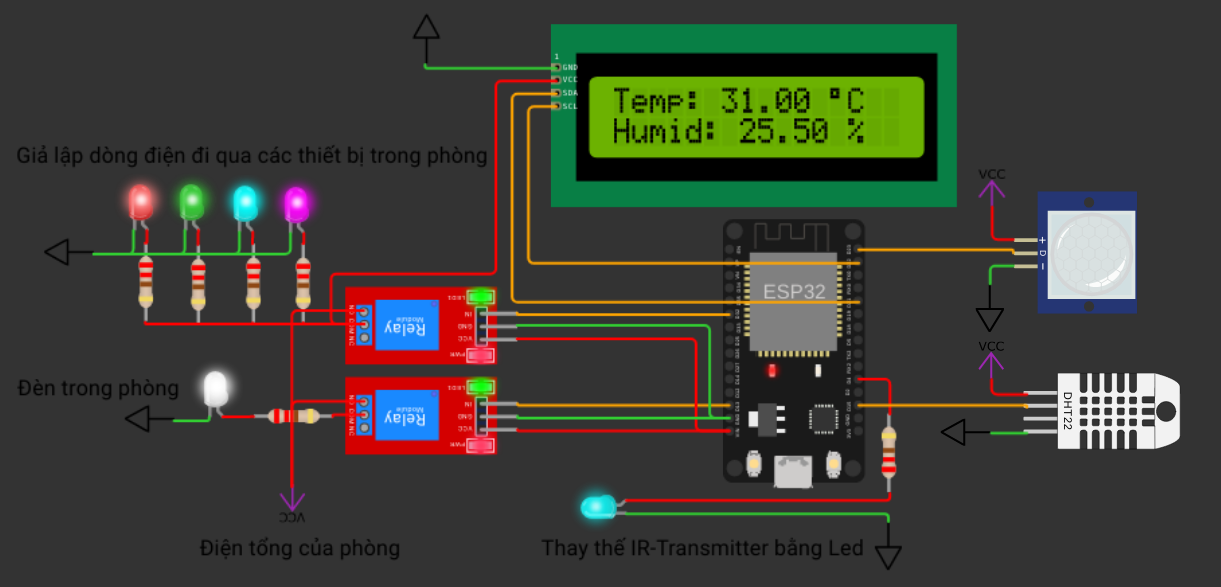
\includegraphics[width=\textwidth, keepaspectratio]{img/mlanh_mo.png}
        \caption{Đèn led màu xanh đại diện cho IR-Transmitter sáng tức là đã phát tín hiệu hồng ngoại}
    \end{figure}

    \item Sau khi không còn ai trong phòng thì các thiết bị sẽ được tắt sau 1 khoảng thời gian nhất định, cụ thể  \textbf{máy lạnh} sẽ được tắt sau khoảng 30 phút tính từ thời điểm không có người nào trong phòng, còn \textbf{các thiết bị khác} sẽ tắt sau khoảng 2 phút.

    \item Đối với trường hợp \textbf{"Bảo vệ"}, các thiết bị trong phòng sẽ không được cung cấp nguồn điện, và khi có người vào trong phòng, sản phẩm sẽ cảnh báo về \textbf{chat bot telegram} rằng có người vào phòng.

    \item Ngoài ra, nhóm đã thiết lập cho phép thay đổi 2 chế độ này thông qua các lệnh được cài đặt trong khung chat bot của telegram, giúp người dùng có thể thay đổi nhanh chóng.
\end{itemize}


\newpage
\subsection{Thiết kế 3D sản phẩm của nhóm}
Dưới đây sẽ là chi tiết về hình ảnh của sản phẩm được thiết kế 3D ở nhiều góc độ.
\begin{itemize}
    \item Đầu tiên phải nói tới vị trí đặt thiết bị ở trong phòng. Nhóm đã thiết kế bố trí sản phẩm ngay phía bên trái của cửa phòng để có thể nhận diện nhanh nhất khi có người vào phòng.
    \begin{figure}[!h]
        \centering
        \includegraphics[width=\textwidth, keepaspectratio]{img/PhoiCanh-01.png}
        \caption{Vị trí đặt thiết bị ở trong phòng}
    \end{figure}

    % \item Đến với chi tiết của sản phẩm, trước hết các thiết bị của sản phẩm được liên kết với nhau và đặt trong hộp làm bằng hộp nhựa acrylic. Bên ngoài của hộp là 2 thiết bị \textbf{Cảm biến chuyển động} và \textbf{màn hình LCD} để người dùng dễ dàng nhìn thấy thông số trong phòng và giúp thiết bị cảm nhận người trong phòng tốt nhất.
    \begin{figure}[!ht]
        \centering
        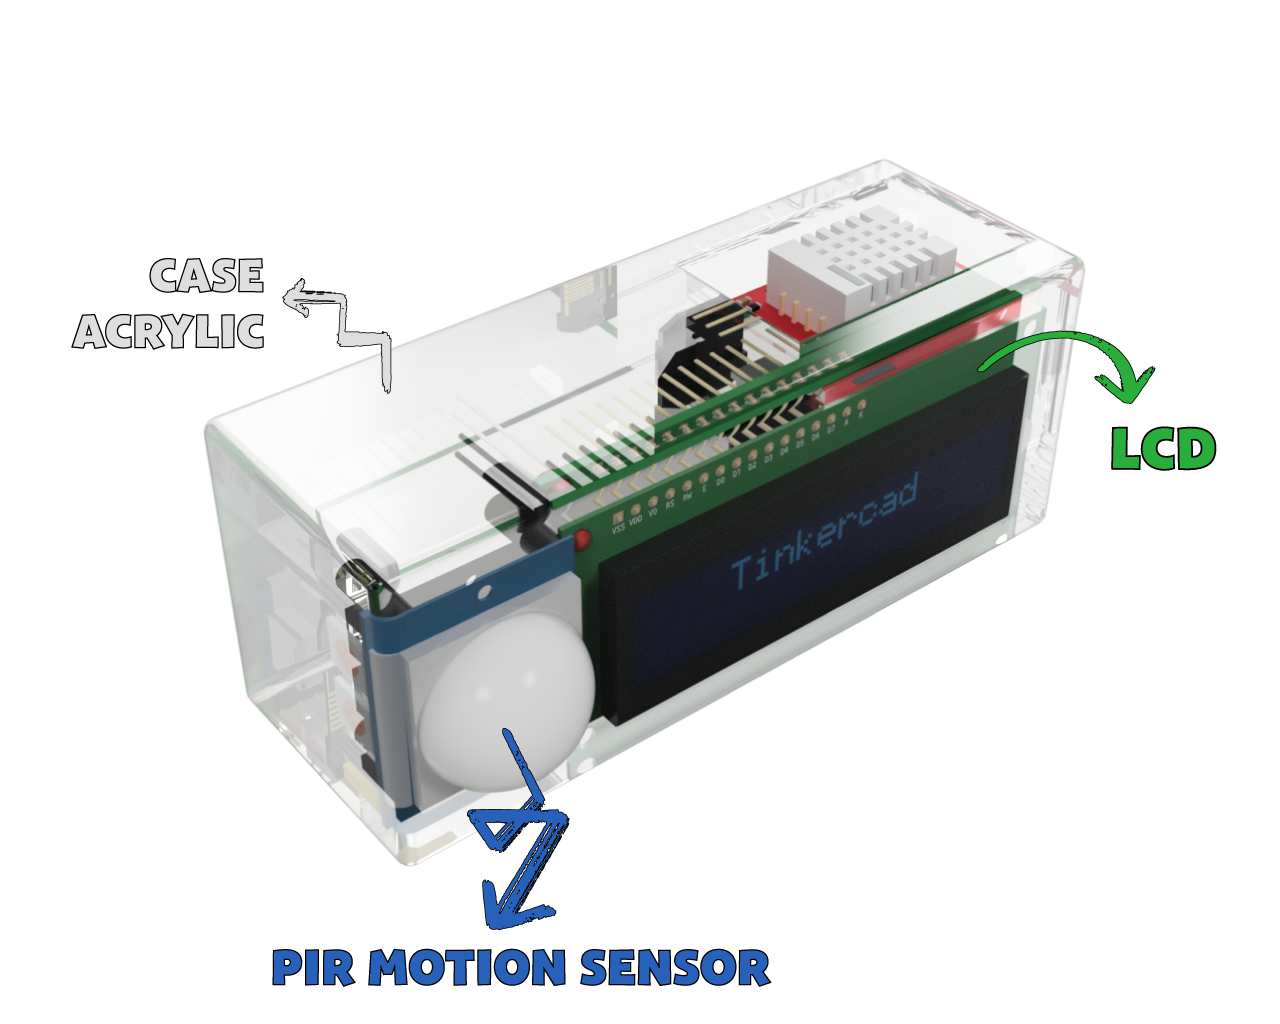
\includegraphics[width=\textwidth, keepaspectratio]{img/1-01.png}
        \caption{Mặt trước của sản phẩm}
    \end{figure}

    % \item Phía trên của sản phẩm chính là thiết bị \textbf{DHT22} dùng để  đo nhiệt độ, độ ẩm. Thiết bị này sẽ kết nối với \textbf{LCD} và thông tin nhiệt độ, độ ẩm sẽ in ra màn hình.
    \begin{figure}[!ht]
        \centering
        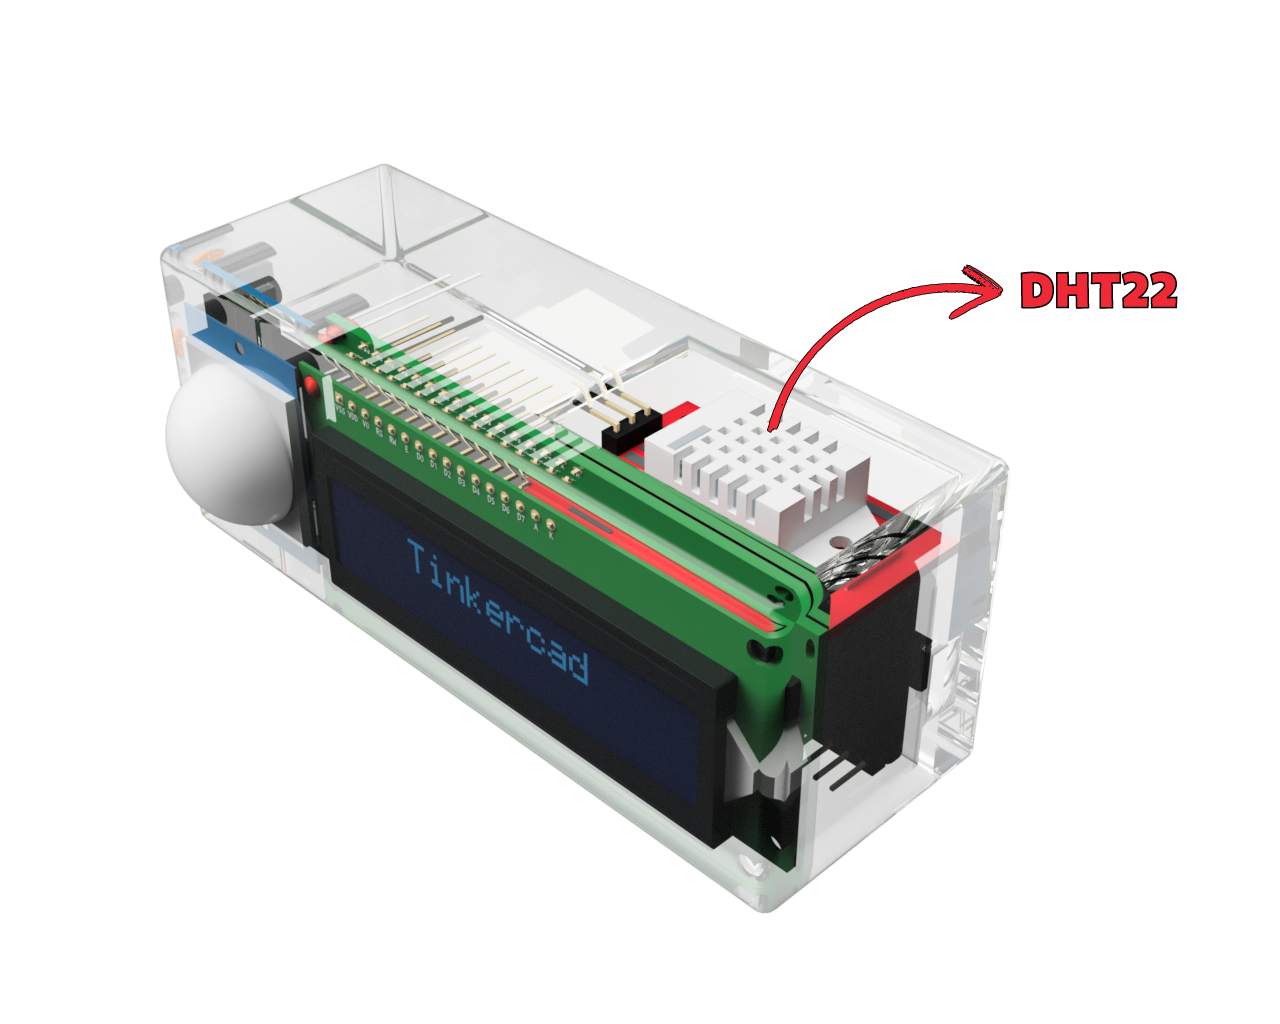
\includegraphics[width=\textwidth, keepaspectratio]{img/2-01.png}
        \caption{Mặt trên của sản phẩm}
    \end{figure}
\end{itemize}

\newpage
\subsubsection{Các tình huống}
\begin{enumerate}
    \item \textbf{Khởi tạo mặc định}: Ban đầu sẽ luôn ở chế độ "ở nhà" và chờ người dùng nhập thiết bị tài khoản và mật khẩu để kết nối với wifi trong khoảng thời gian 5 phút. Nếu sau 5 phút không có kết nối wifi thì sẽ hoạt động với trường hợp \textbf{Sự cố mạng} bên dưới.

    \item \textbf{Sự cố mạng}: Người dùng không thể truy cập và chỉnh sửa chế độ từ xa, các thiết lập được chuyển về chế độ "ở nhà" (Ưu tiên trải nghiệm người dùng hơn tiết kiệm điện). 
    
    \item \textbf{Cúp điện đột ngột}: Trường hợp bất khả kháng của nhà cung cấp điện, ngay khi có điện trở lại thì sẽ về chế độ \textbf{khởi tạo mặc định}.
\end{enumerate}

\newpage
\section{Tài liệu tham khảo}
\begin{itemize}
    \item 
    \href{https://www.youtube.com/watch?v=eODatazcbaw}{Ý tưởng kết nối DHT11 và ESP32}

    \item
    \href{https://wokwi.com/projects/300028989690348041}{Ý tưởng thiết kế IR receiver}
    
    \item \href{https://tex.stackexchange.com/questions/125135/insert-pages-from-a-pdf-file-to-fit-at-the-entire-page-using-includepdf}{Fitpaper}

    \item \href{https://hshop.vn}{HShop - shop linh kiện điện tử \& Robot}

    \item \href{https://hshop.vn/products/cam-bien-do-am-nhiet-do-dht11-ra-chan}{Tham khảo giá `DHT11'}
    \item \href{https://hshop.vn/products/cam-bien-sieu-am-srf04}{Tham khảo giá `Cảm biến siêu âm'}
    \item \href{https://hshop.vn/products/mat-thu-hong-ngoai-1838}{Tham khảo giá 'mắt đọc hồng ngoại'}
    \item \href{https://hshop.vn/products/lcd-text-lcd1602-xanh-duong}{Tham khảo giá 'LCD'}
    \item \href{https://hshop.vn/products/mach-relay-tre-ic555}{Tham khảo giá `Relay'}
    \item \href{https://hshop.vn/products/dieu-khien-hong-ngoai-ir-remote-control-38khz}{Tham khảo giá 'điều khiển hồng ngoại'}
    \item \href{https://hshop.vn/products/kit-rf-thu-phat-wifi-ble-esp32-s2-nodemcu-32-s2-ai-thinker}{Tham khảo giá 'Board ESP32'}

    \item \href{https://hshop.vn/products/arduino-uno-r3}{Tham khảo giá 'Arduino uno r3' (kèm cáp USB 30cm)}
    \item \href{https://hshop.vn/search?type=product&q=dây%20cắm}{Tham khảo giá `Dây cắm'}
    \item \href{https://dientutuonglai.com/nguon-adapter-5v1a-dau-ra-day-nguon-usb-va-dc5-5.html}{Tham khảo giá `nguồn 5V - 1A cho Arduino'}

    \item \href{https://shp.ee/zau4d86}{Tham khảo giá 'hộp mica'}
    
\end{itemize}
% ========== END [MAIN CONTENT] ==========
\end{document}